\section{Implementation}

\subsection{Repository}
The source code as well as the Latex code for this PDF is publicly available in the GitHub repository: \url{https://github.com/piniom/partition}. \\
The Latex source code is automatically compiled using GitHub Actions and the resulting PDF is available in the \texttt{releases} section of the repository.

\subsection{Programming Language}
The Rust Programming Language was chosen for this project due to its known performance and safety characteristics \cite{rust_cpp}.

\subsubsection{Outside dependencies}
This project uses the following external libraries:
\begin{itemize}
    \item \texttt{rustfft\footnote{\url{https://github.com/ejmahler/RustFFT}}} - a Fast Fourier Transform library.
    \item \texttt{concrete-ntt\footnote{\url{https://github.com/zama-ai/concrete-ntt}}} - a Discrete Fourier Transform library.
    \item \texttt{clap\footnote{\url{https://github.com/clap-rs/clap}}} - a command line argument parser.
\end{itemize}
Additionally, the following libraries are used for testing:
\begin{itemize}
    \item \texttt{rand\footnote{\url{https://github.com/rust-random/rand}}} - a library for random number generation. 
    \item \texttt{proptest\footnote{\url{https://github.com/proptest-rs/proptest}}} - a library for property-based testing.
\end{itemize}

\subsubsection{Rust Standard Library}
Apart from the external libraries, the Rust Standard Library is used extensively.

\subsection{Usage}
The project is both a rust library and a command line application. 
\subsubsection{Library}
The library can be used by adding a git dependency to the \texttt{Cargo.toml} file of the project.
\subsubsection{Command Line Application}
The command line application can be built using the \texttt{cargo} tool. The application takes a list of integers and the approximation coefficient as input and outputs the approximate solution to the \Partition problem. The application can be run with the \texttt{--help} flag to see the available options.

\subsection{Tests}
The project is tested extensively using both unit tests and property-based testing. When testing the set of subset sums approximation, for small inputs, where the exponential complexity is acceptable, the output of the algorithm is compared to the output of the naive algorithm. For larger inputs, I test that the approximated set of subset sums contains some arbitrary subset sum.

\subsection{Benchmarks}
\begin{figure}[h!]
    \centering
    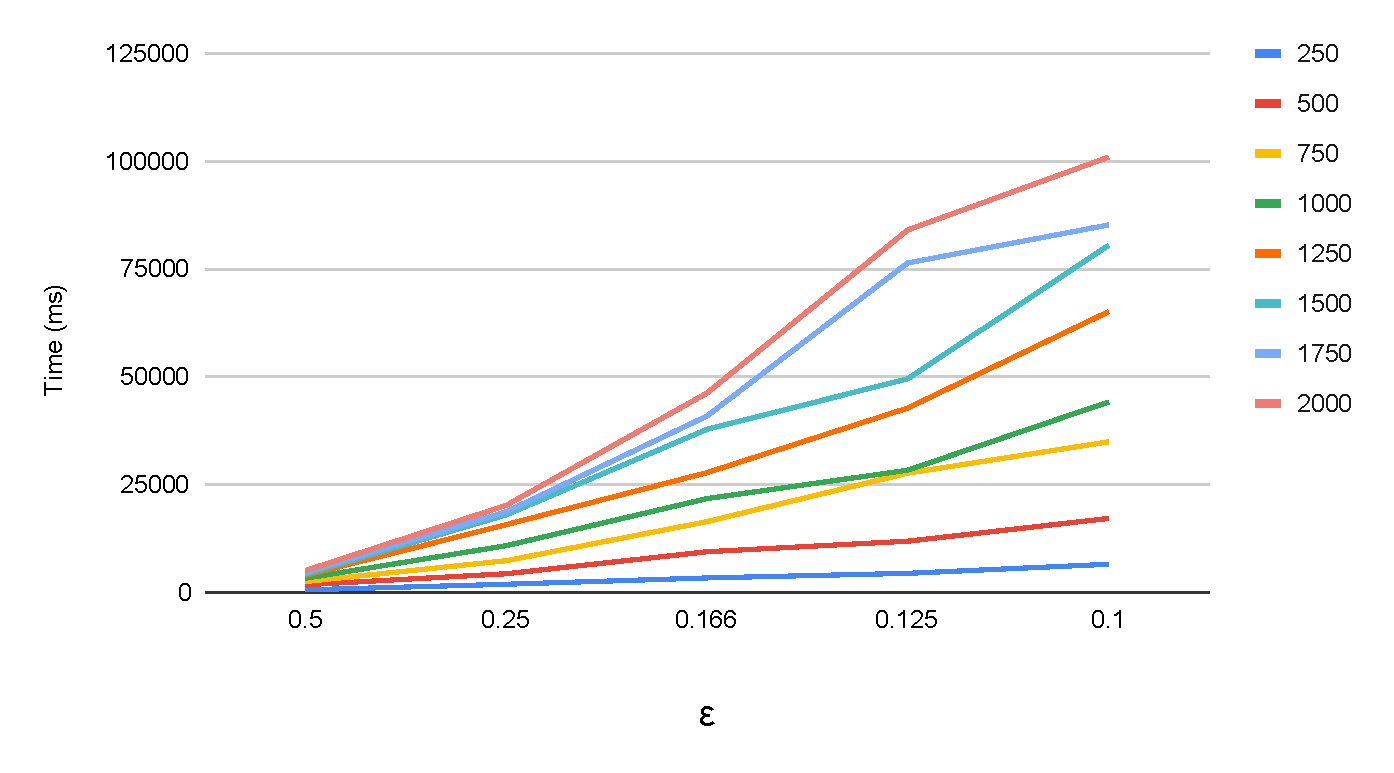
\includegraphics[width=\linewidth]{charts/epsilon.pdf}
    \caption{Running time parameterised by $\varepsilon$ for different input lengths.}
    \label{fig:chart}
\end{figure}

\begin{figure}[h!]
    \centering
    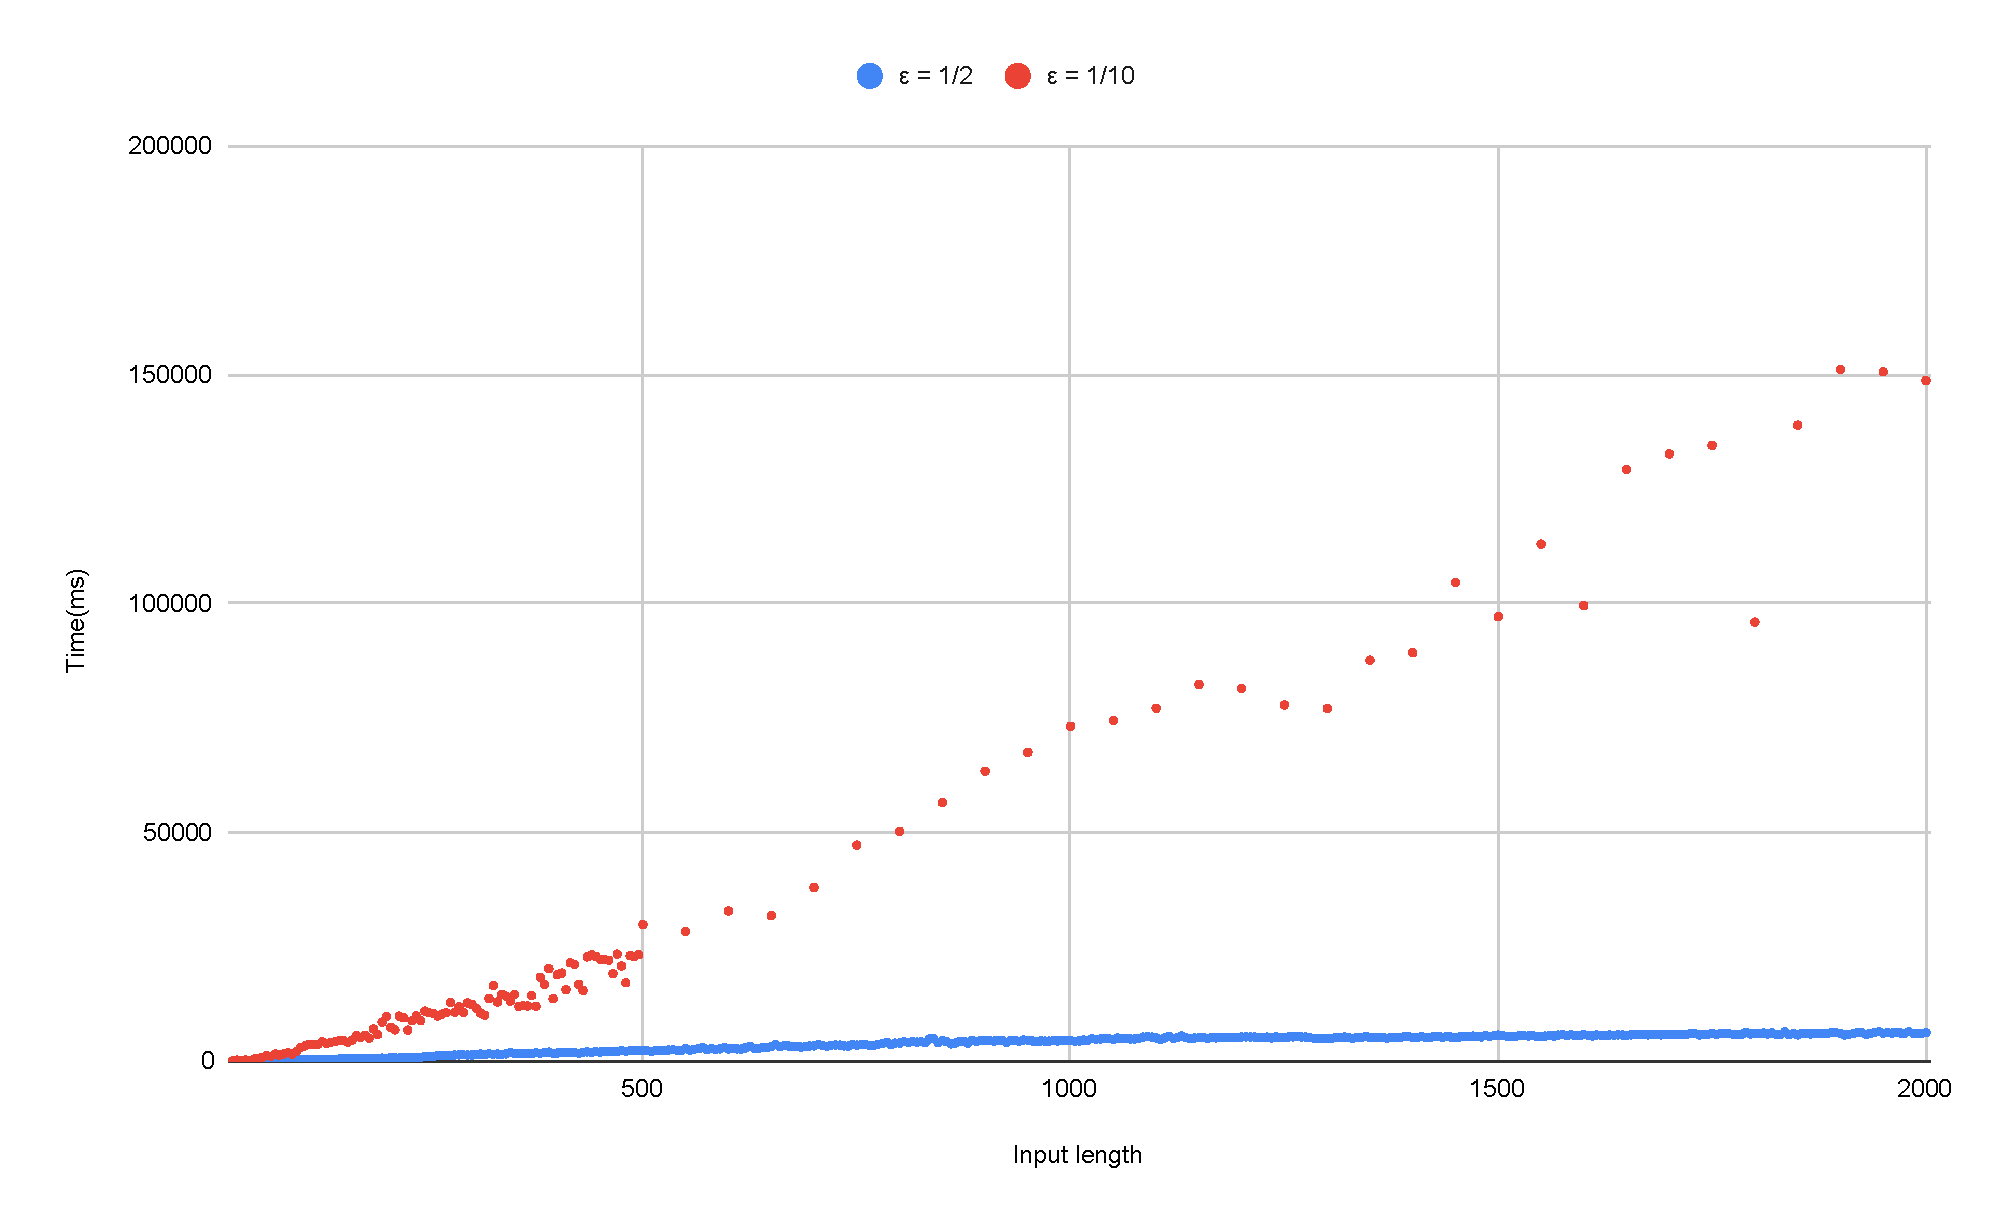
\includegraphics[width=\linewidth]{charts/input_length.pdf}
    \caption{Running time for different input lengths, parameterised by $\varepsilon$.}
    \label{fig:chart}
\end{figure}

\begin{figure}[h!]
    \centering
    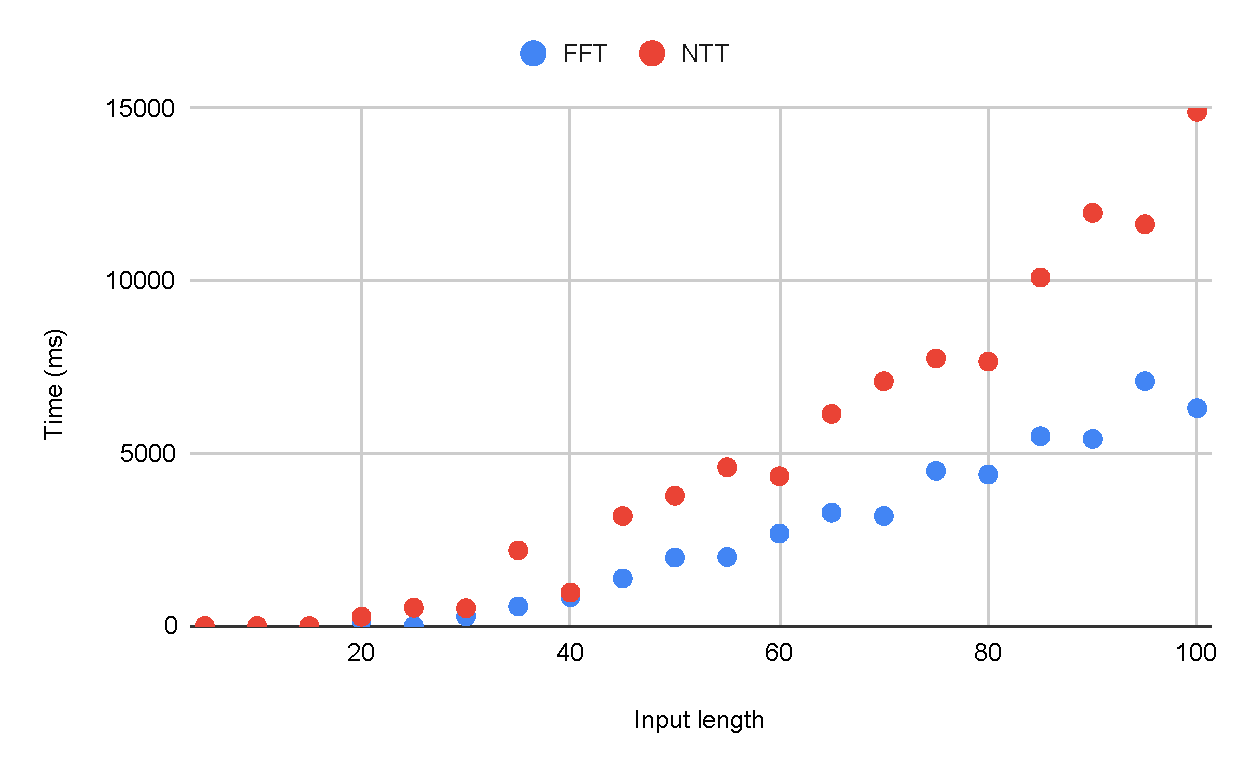
\includegraphics[width=\linewidth]{charts/fft_ntt.pdf}
    \caption{Comparison of the running time of the approximation using the FFT and NTT as convolution backends with $\varepsilon = 1/25$  }
    \label{fig:chart}
\end{figure}

\begin{figure}[h!]
    \centering
    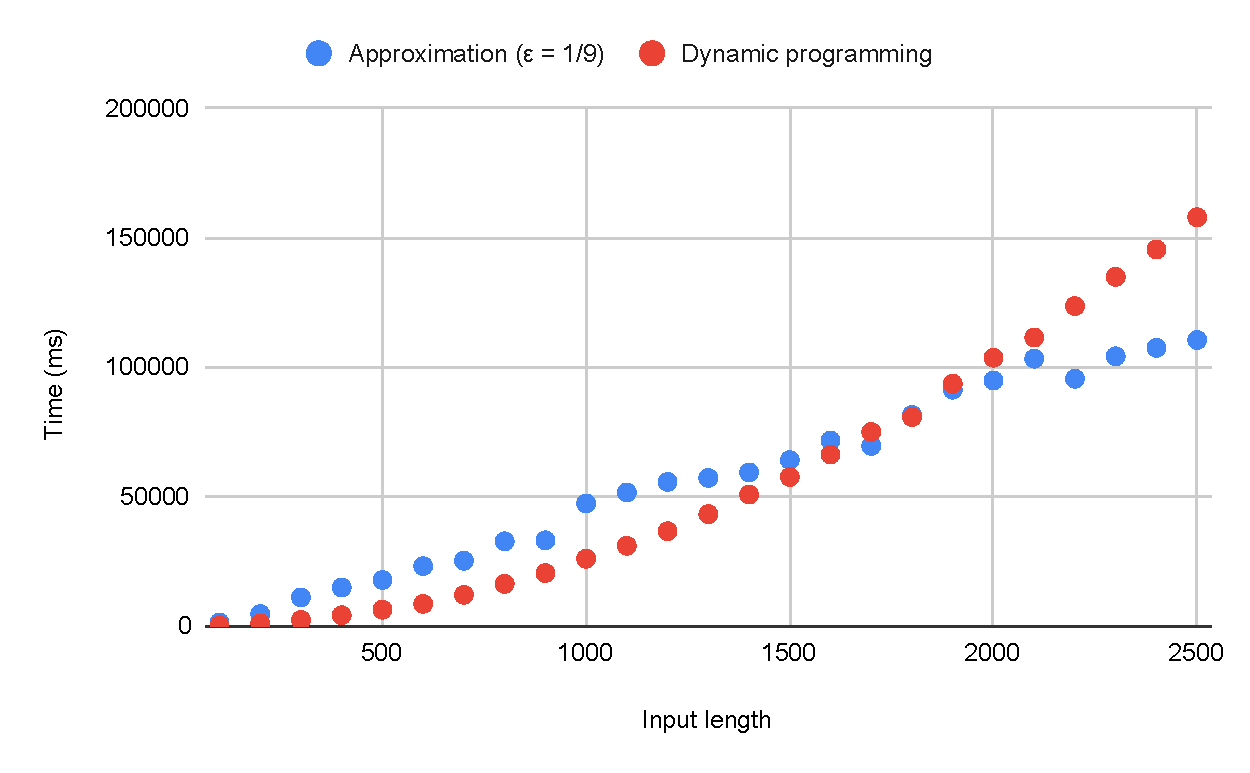
\includegraphics[width=\linewidth]{charts/dp.pdf}
    \caption{Running time of the approximation with $\varepsilon = 1/9$ compared to a dynamic-programming.}
    \label{fig:chart}
\end{figure}


\begin{figure}[h!]
    \centering
    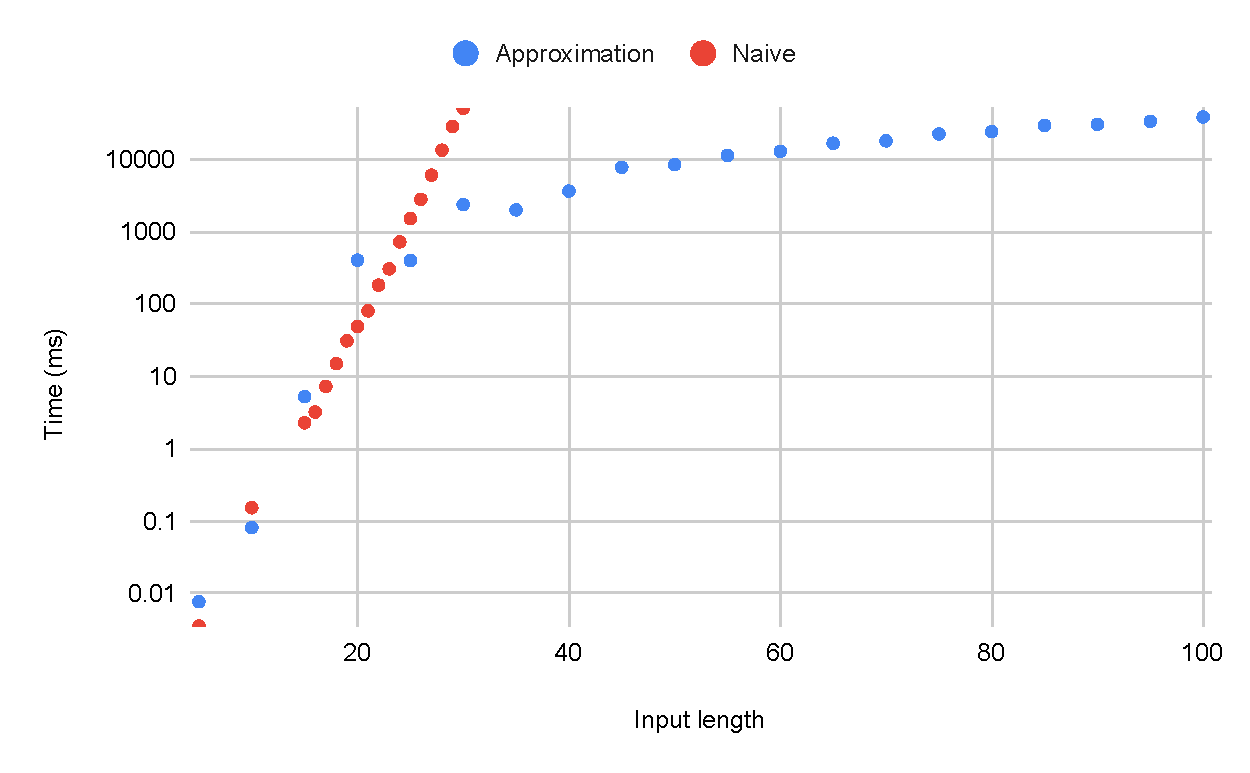
\includegraphics[width=\linewidth]{charts/naive.pdf}
    \caption{Running time of the approximation with $\varepsilon = 1/100$ compared to a naive algorithm on a logarithmic scale.}
    \label{fig:chart}
\end{figure}


